\documentclass[11pt, oneside]{article} 
\usepackage{geometry}
\geometry{letterpaper} 
\usepackage{graphicx}
	
\usepackage{amssymb}
\usepackage{amsmath}
\usepackage{parskip}
\usepackage{color}
\usepackage{hyperref}

\graphicspath{{/Users/telliott/Github/precalculus/fig/}}
% \begin{center} \includegraphics [scale=0.4] {gauss3.png} \end{center}

\title{Connecting all four points}
\date{}

\begin{document}
\maketitle
\Large
\subsection*{orthocenter}
An altitude of a triangle is a line extended from a vertex so as to form a right angle with the opposing side.  The \emph{orthocenter} is the point where the three altitudes of a triangle meet.

Assume for now that the three altitudes \emph{do} meet at a single point, we will come back to this question later.
\begin{center} 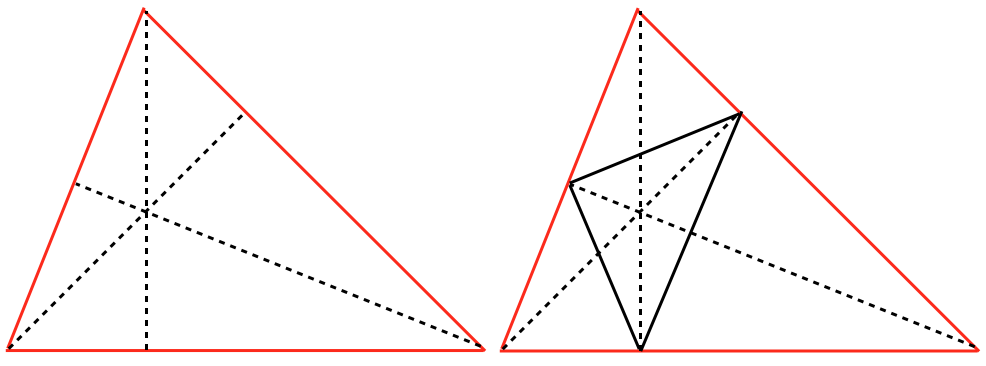
\includegraphics [scale=0.4] {altitude_proof_1.png} \end{center}

Above we have drawn the altitudes (left panel) and connected the points where the altitudes meet the sides.  We can prove something interesting about the inset triangle.  We will prove that the incenter of that triangle is equal to the orthocenter of the bigger one.

\begin{center} 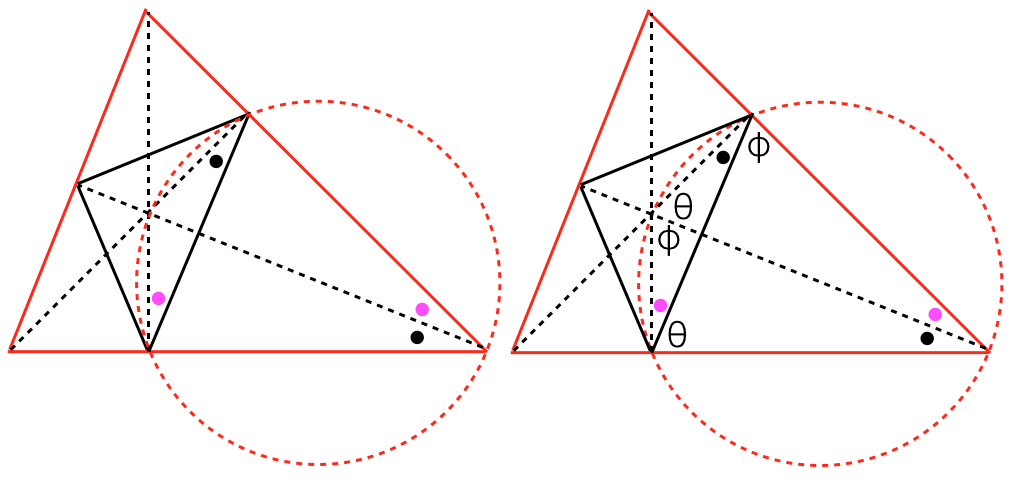
\includegraphics [scale=0.4] {altitude_proof_2.png} \end{center}

The dotted lines form right angles at the sides.  Therefore, we can use the common dotted line as a diameter and draw a circle that includes all four points.

Despite what it looks like, the figure is not symmetrical across the diameter.  For example, the angles marked with black dots and those marked with magenta dots are not equal.

However, now we can use our theorems about arcs subtended by an angle on the perimeter of the circle.  The two angles marked with black dots subtend the same arc.  Similarly for magenta.  The same is also true for the pairs of angles marked $\phi$ and $\theta$.

We use symmetry to fill in some more equalities.

\begin{center} 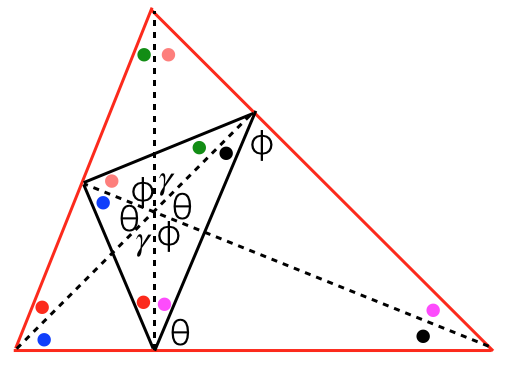
\includegraphics [scale=0.4] {altitude_proof_3.png} \end{center}

This looks like a mess.  But let us look more carefully at one set of angles, $\phi$ and the black and green.

\begin{center} 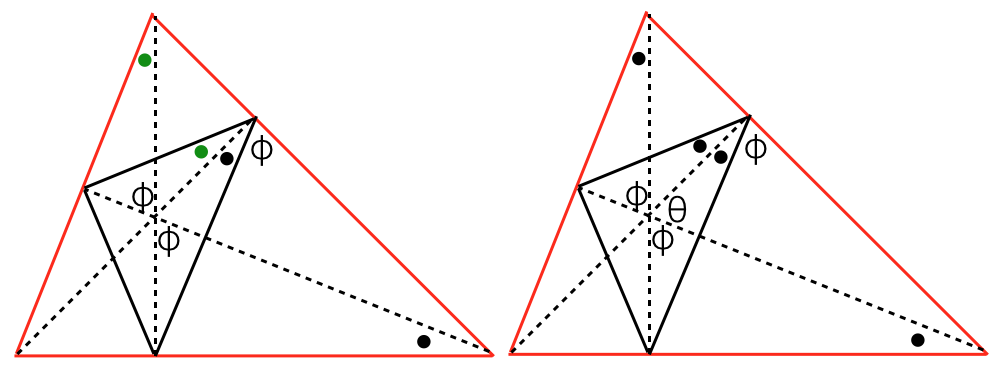
\includegraphics [scale=0.4] {altitude_proof_4.png} \end{center}

Notice that, at the bottom, $\phi$ is complementary to black, but the top left, $\phi$ is complementary to green.  Hence black and green must be equal (right panel).  We carry out the same exercise for $\theta$, red and pink.

\begin{center} 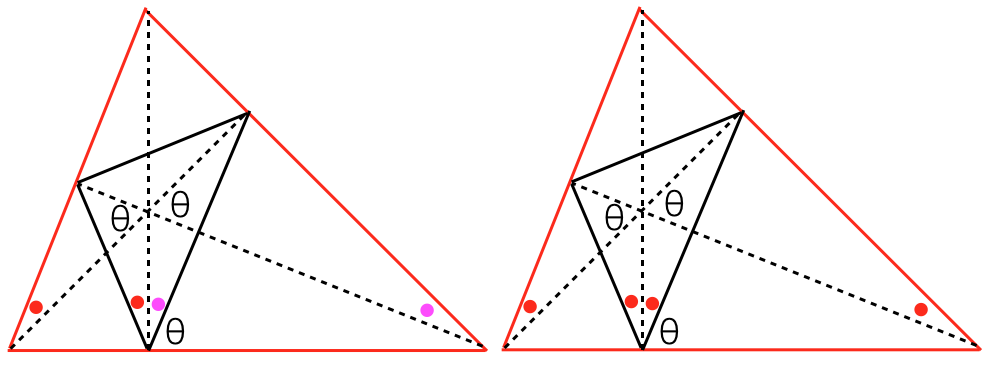
\includegraphics [scale=0.4] {altitude_proof_5.png} \end{center}

And then, for $\gamma$, blue and salmon.
\begin{center} 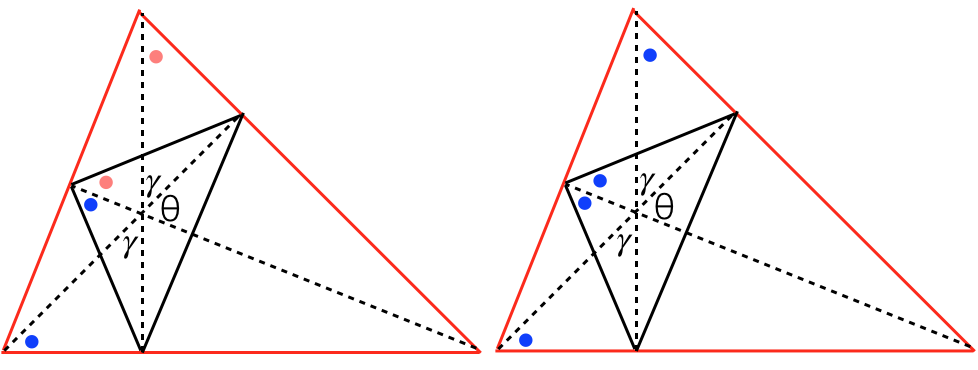
\includegraphics [scale=0.4] {altitude_proof_6.png} \end{center}

Restoring dots
\begin{center} 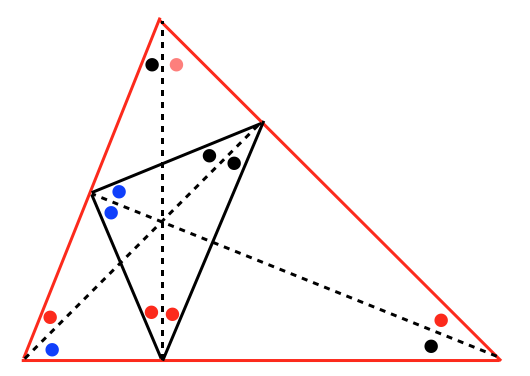
\includegraphics [scale=0.4] {altitude_proof_7.png} \end{center}

We can see that the dotted lines are angle bisectors for the small triangle.

Thus, the orthocenter of the large triangle and the incenter of the triangle inscribed between the points along the base, are the same point.

$\square$

\subsection*{Orthocenter exists}
Because we can (and have already) extended Ceva's general proof to the specific case of the orthocenter (altitudes meeting at a point), we don't need a specific proof.  Nevertheless, it's good practice.  Here is a nice short one.

\begin{center} 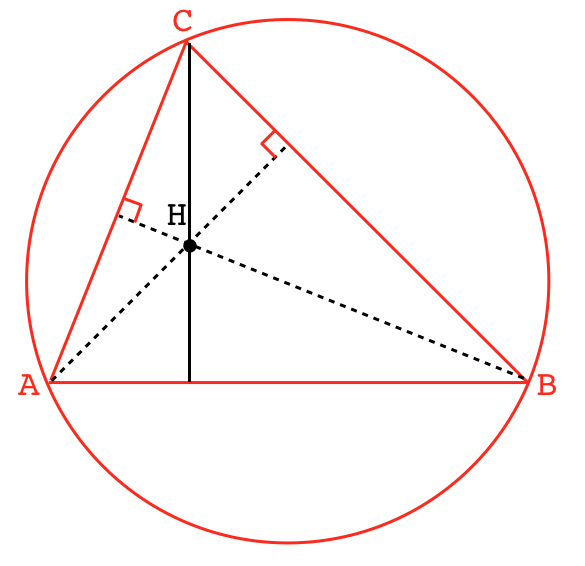
\includegraphics [scale=0.35] {ortho4.png} \end{center}

We have $\triangle ABC$, with two altitudes drawn (and marked as right angles where they hit the sides), and a third line from vertex $C$ that we need to show makes a right angle with side $AB$.  We've also drawn the circumcircle of the triangle.

\begin{center} 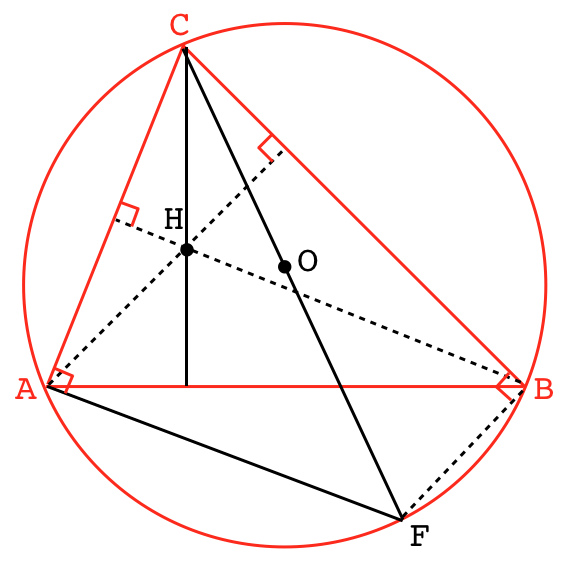
\includegraphics [scale=0.35] {ortho5.png} \end{center}

Draw the diameter of the circle, and form right angles at vertexes $A$ and $B$ by inscribing a right triangle as each.

Since $AH$ is on a line that forms a right angle with $BC$ and so is $BF$, we have that $AH$ is parallel to $BF$.  Similarly, $BH$ is parallel to $AF$, so $AHBF$ is a parallelogram.

We draw the other diameter of the parallelogram.
\begin{center} 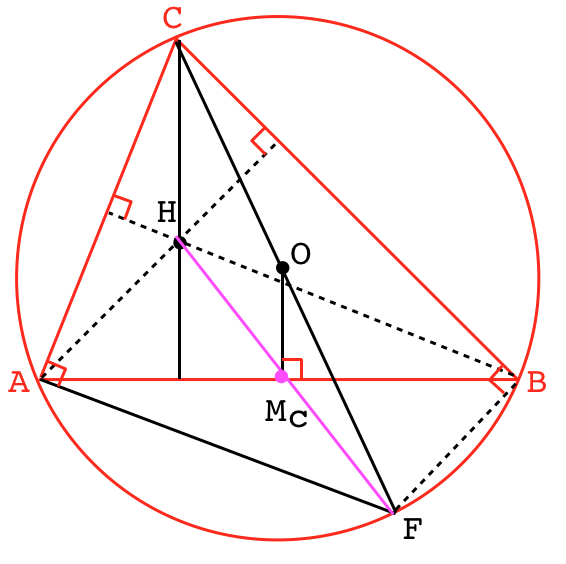
\includegraphics [scale=0.35] {ortho6.png} \end{center}

Diameters of a parallelogram cross at their midpoints.  Therefore, $AM_c = M_c B$ and so the line from the center to $M_c$ is a perpendicular bisector of $AB$.  As well, $HM_c = M_cF$.

Because $CO = OF$ and $HM_c = M_c F$, $OM_c$ is a \emph{midline} of $\triangle CHF$

Therefore, $\triangle CHF$ is similar to $\triangle OM_cF$.  As a result, $CH$ is parallel to $OM_c$.

Therefore its extension forms a right angle with $AB$, just as $OM_c$ does.

$\square$

\subsection*{Euler's proof}

Below we give a third proof.  This one, due to Euler, is stunning.  It follows:

\url{https://artofproblemsolving.com/wiki/index.php/Orthocenter}

A copy of their figure:

\begin{center} 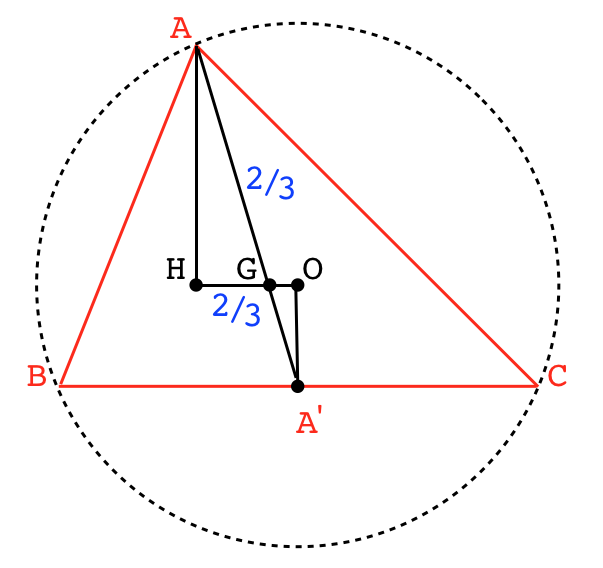
\includegraphics [scale=0.35] {circumcenter4.png} \end{center}
The orientation is reversed from what we had above.  First, the point $O$ is the circumcenter of the triangle:  the center of the circle which contains all three vertices of the triangle.  

Clearly, this circle  has a center.  The classic construction is to bisect each side (here $BC$ is bisected at $A'$), and erect a perpendicular.  The point where the three perpendiculars cross is the circumcenter, which is the center of the circle.  

\begin{center} 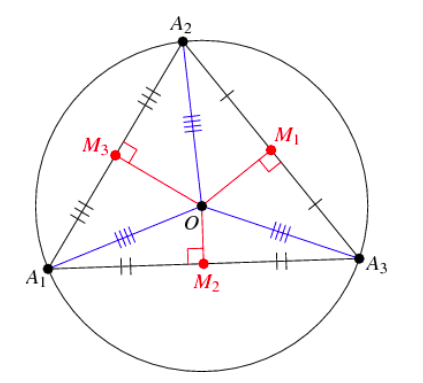
\includegraphics [scale=0.45] {three_point_circle2.png} \end{center}

So, assume we have done this and that point is $O$.

The next point, $G$, is the centroid.  One way to find this point is to draw all three lines connecting vertices with the midpoints of the opposite side ($AA'$).  However, if you recall, the distance from the vertex $A$ to $G$ is twice the distance from the midpoint $A'$ to $G$.  Hence we draw point $G$ using arithmetic.

Now, extend $OG$ by twice its length, to $H$.  ($2OG = GH$).
\begin{center} 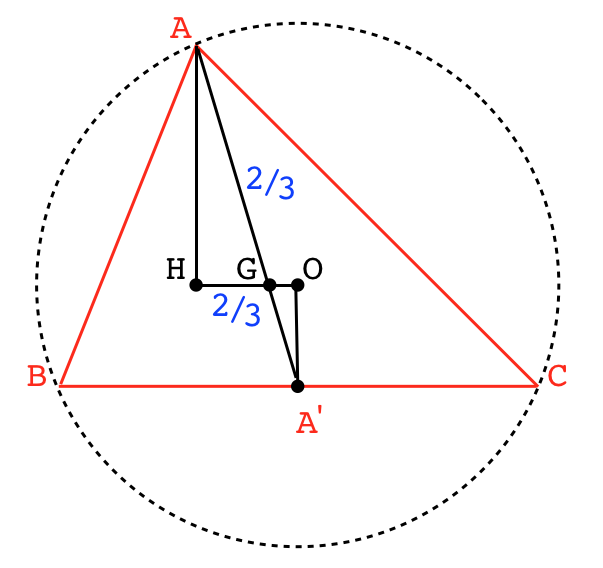
\includegraphics [scale=0.35] {circumcenter4.png} \end{center}
Because $AG$ is twice $A'G$ and $GH$ is twice $OG$ and the two triangles share both angle $\angle OGA'$ (equal to $\angle AGH$), they are similar triangles.  

Since $\angle A'OG$ is a right angle, therefore so is $\angle AHG$.  This means that $AH$ is perpendicular to $BC$.  Thus, $AH$ is a part of the altitude from $A$ to $BC$ (the whole altitude is not shown).

The same construction could be done for the other two vertices, each time ending at $H$.  This shows that $H$ is unique, and that $H$ is on all three altitudes.

This proof also demonstrates that the orthocenter, centroid and circumcenter lie on a single line, and that the distance from centroid to orthocenter is twice that from centroid to circumcenter.


\end{document}